\chapter{Latent Heat of Vaporization of Liquid Nitrogen}

Date: 5/11/2020

\section{Aim}
The aim of this experiment is to understand latent heat of vaporization through liquid nitrogen and safe use of cryogens through a setup of circuits for heating and measurement of current and voltage through liquid nitrogen. 


\section{Background Theory}

Latent heat is defined as energy released or absorbed when a substance changes state. Latent heat absorbed when a solid changes to liquid is latent heat of fusion. Latent heat absorbed when a liquid changes to vapour, to break inter-molecular forces, is known as latent heat of vaporisation. It can be calculated using 
$$ L_v = \frac{\triangle Q}{\triangle m}$$ 
where Q is amount of energy and m is mass. 
Liquid Nitrogen is an odourless and a colourless fluid that starts to evaporate at room temperature


\section{Description of Setup}
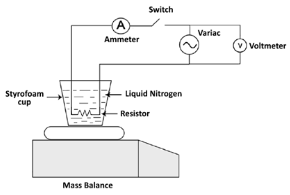
\includegraphics[width=10cm, height=7cm]{figures/image.png} \\
Using the setup above, a resistor is attached to variac through an ammeter in series. Liquid Nitrogen is used in a Styrofoam cup to isolate it thermally to calculate latent heat. An electronic balance is used to measure the change in mass of nitrogen as it is heated.  


\section{Method / Procedure}
The apparatus was set up and liquid nitrogen was poured from a cryogenic container into the Styrofoam cup using gloves and safety goggles. The mass of the cup with resistor inside was measured and the mass lost is measured. Start the stopwatch timer and wait for 20 seconds. Note mass for every second for 30 seconds. Start the variac and heater which increases the rate of mass loss. The mass was recorded for every second for 30 seconds. The heating was then turned off for 30 seconds and mass recorded. The previous two steps are repeated one more time. At the end, the cup is removed and leftover liquid nitrogen is poured back.


\section{Data}
The type B uncertainty associated with time is 0.003s. The type B uncertainty associated with Mass is 0.03 g.  

\begin{center}
\begin{adjustbox}{width=1\textwidth}
\begin{tabular}{|l|l|l|l|l|l|l|l|l|}
\hline
     & \multicolumn{2}{c|}{heating off 1} & \multicolumn{2}{c|}{heating on 1} & \multicolumn{2}{c|}{heating off 2} & \multicolumn{2}{c|}{heating on 2} \\ \hline
s.No & time (s)      & Mass   (grams)     & time (s)     & Mass   (grams)     & time (s)      & Mass   (grams)     & time (s)     & Mass   (grams)     \\ \hline
1  & 20 & 90.2 & 50 & 88.8 & 80  & 83.6 & 110 & 82.6 \\ \hline
2  & 21 & 90.0 & 51 & 88.7 & 81  & 83.6 & 111 & 82.6 \\ \hline
3  & 22 & 89.9 & 52 & 88.7 & 82  & 83.6 & 112 & 82.6 \\ \hline
4  & 23 & 89.9 & 53 & 88.5 & 83  & 83.4 & 113 & 82.4 \\ \hline
5  & 24 & 89.8 & 54 & 88.3 & 84  & 83.4 & 114 & 82.2 \\ \hline
6  & 25 & 89.8 & 55 & 88.1 & 85  & 83.4 & 115 & 82.1 \\ \hline
7  & 26 & 89.8 & 56 & 88.0 & 86  & 83.4 & 116 & 81.9 \\ \hline
8  & 27 & 89.7 & 57 & 87.7 & 87  & 83.4 & 117 & 81.8 \\ \hline
9  & 28 & 89.6 & 58 & 87.7 & 88  & 83.4 & 118 & 81.6 \\ \hline
10 & 29 & 89.6 & 59 & 87.3 & 89  & 83.4 & 119 & 81.5 \\ \hline
11 & 30 & 89.5 & 60 & 87.2 & 90  & 83.3 & 120 & 81.2 \\ \hline
12 & 31 & 89.5 & 61 & 87.0 & 91  & 83.3 & 121 & 81.1 \\ \hline
13 & 32 & 89.5 & 62 & 86.8 & 92  & 83.2 & 122 & 81.0 \\ \hline
14 & 33 & 89.4 & 63 & 86.7 & 93  & 83.2 & 123 & 80.8 \\ \hline
15 & 34 & 89.4 & 64 & 86.5 & 94  & 83.2 & 124 & 80.6 \\ \hline
16 & 35 & 89.3 & 65 & 86.2 & 95  & 83.1 & 125 & 80.4 \\ \hline
17 & 36 & 89.3 & 66 & 86.2 & 96  & 83.1 & 126 & 80.2 \\ \hline
18 & 37 & 89.3 & 67 & 85.9 & 97  & 83.0 & 127 & 80.0 \\ \hline
19 & 38 & 89.2 & 68 & 85.8 & 98  & 83.0 & 128 & 80.0 \\ \hline
20 & 39 & 89.2 & 69 & 85.6 & 99  & 83.0 & 129 & 79.8 \\ \hline
21 & 40 & 89.2 & 70 & 85.4 & 100 & 83.0 & 130 & 79.6 \\ \hline
22 & 41 & 89.0 & 71 & 85.2 & 101 & 82.9 & 131 & 79.6 \\ \hline
23 & 42 & 89.0 & 72 & 85.2 & 102 & 82.9 & 132 & 79.4 \\ \hline
24 & 43 & 89.0 & 73 & 84.9 & 103 & 82.9 & 133 & 79.2 \\ \hline
25 & 44 & 89.0 & 74 & 84.8 & 104 & 82.8 & 134 & 79.0 \\ \hline
26 & 45 & 89.0 & 75 & 84.6 & 105 & 82.8 & 135 & 78.8 \\ \hline
27 & 46 & 88.9 & 76 & 84.5 & 106 & 82.8 & 136 & 78.8 \\ \hline
28 & 47 & 88.9 & 77 & 84.2 & 107 & 82.8 & 137 & 78.7 \\ \hline
29 & 48 & 88.8 & 78 & 84.1 & 108 & 82.8 & 138 & 78.5 \\ \hline
30 & 49 & 88.8 & 79 & 83.9 & 109 & 82.6 & 139 & 78.3 \\ \hline
\end{tabular}
\end{adjustbox}
\end{center}


% In this section, describe what data was recorded during the experiment. Mention which quantities are being measured, which quantity is independent, which is dependent and which are constants. Make this difference very explicit. Make sure to quantify and state the uncertainties in the recorded data. Be precise and primarily include numerical data.

\section{Data Analysis}

Rate of Change Mass at different times 
\begin{center}
\begin{tabular}{|l|l|}
\hline
Time            & Rate of Change of Mass (g/s) \\ \hline
Heating  Off 1  & -0.04349                     \\ \hline
Heating   On 1  & -0.1744                      \\ \hline
Heating   Off 2 & -0.03418                     \\ \hline
Heating   On 2  & -0.1562                      \\ \hline
\end{tabular}
\end{center}
The average rate of change in mass when heating is off is $-0.3884 g/s$ and the average of change in mass when heating is on is $ -0.1653 g/s$

% 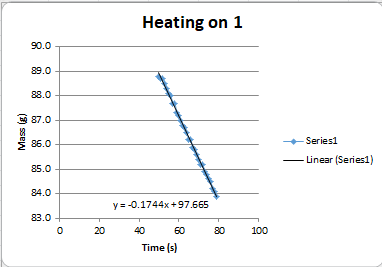
\includegraphics[width=8cm, height=7cm]{figures/on_1.png} \\
% 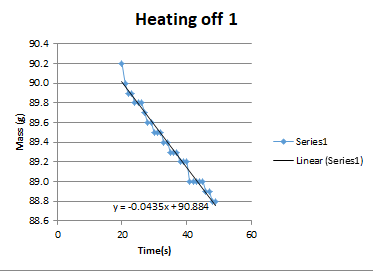
\includegraphics[width=8cm, height=7cm]{figures/off_1.png} \\
% 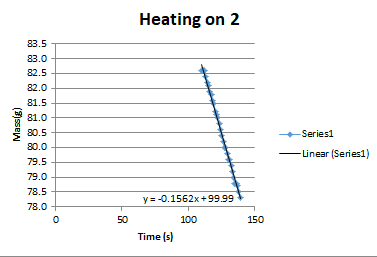
\includegraphics[width=10cm, height=7cm]{figures/on_2.png} \\
% 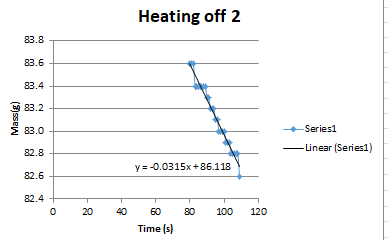
\includegraphics[width=10cm, height=7cm]{figures/off_2.png} \\

% In this section, mention the calculations you perform, uncertainties transferred, and statistical analysis (residuals, errors, uncertainties in parameters fit etc.). Be precise and primarily include numerical data \ref{eq:line}.
\newpage
\begin{figure}[h!]
    \centering
    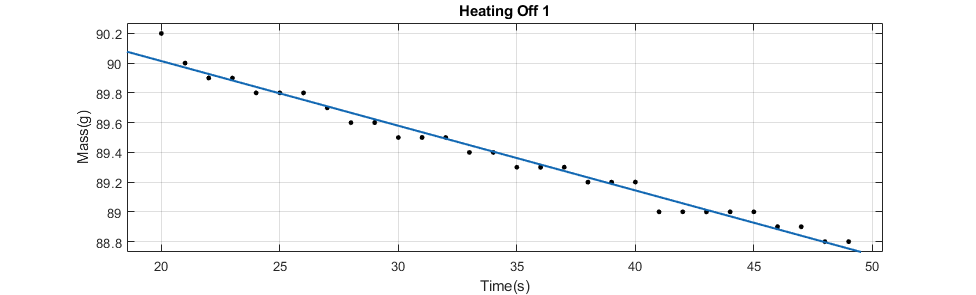
\includegraphics[width=\textwidth]{figures/TimeOff1_c.png}
    \caption{Heating Time Off 1}
    \label{fig:yx}
\end{figure}
The line of best fit : $ y = -0.04389x + 90.88$ \\
\newpage
\begin{figure}[h!]
    \centering
    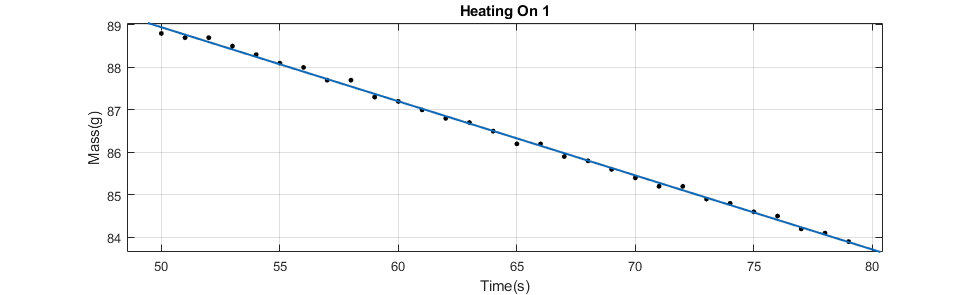
\includegraphics[width=\textwidth]{figures/TimeOn1_c.png}
    \caption{Heating Time On 1}
    \label{fig:yx}
\end{figure}
The line of best fit : $ y = -0.01744x + 97.67$ \\
\newpage
\begin{figure}[h!]
    \centering
    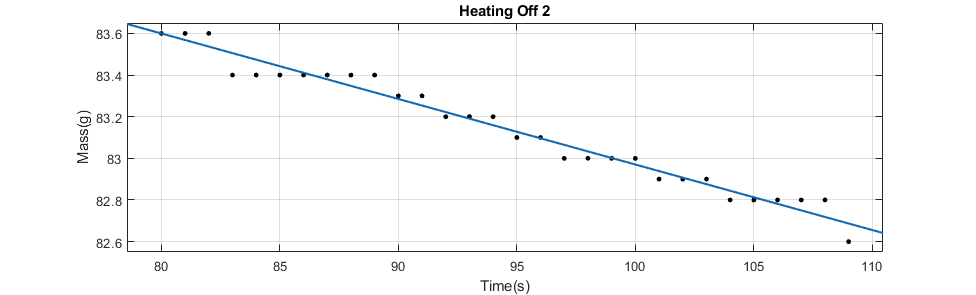
\includegraphics[width=\textwidth]{figures/TimeOff2_c.png}
    \caption{Heating Time Off 2}
    \label{fig:yx}
\end{figure}
The line of best fit : $ y = -0.03418x + 86.12$ \\
\newpage
\begin{figure}[h!]
    \centering
    \includegraphics[width=\textwidth]{figures/TimeOn2_C.png}
    \caption{Heating Time On 2}
    \label{fig:yx}
\end{figure}
The line of best fit : $ y = -0.1562x + 99.99$ \\
\newpage
\begin{figure}[h!]
    \centering
    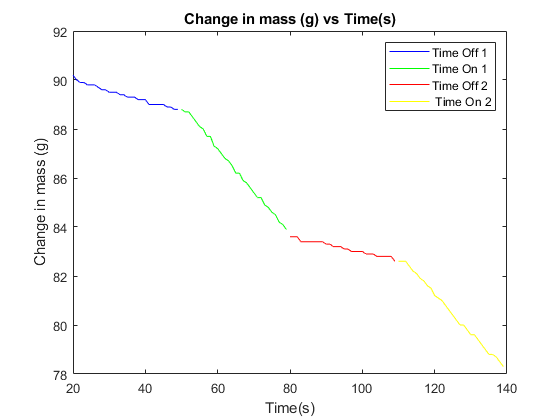
\includegraphics[width=\textwidth]{figures/Final.png}
    \caption{The graph of change in mass vs Time}
    \label{fig:yx}
\end{figure}

Rate of mass lost for electrical heating is calculated using 
\begin{equation}
    \frac{\triangle m}{\triangle t}_{Electric-heating} = \frac{\triangle m}{\triangle t}_{Electric-heating + Ambient-heat} - \frac{\triangle m}{\triangle t}_{Ambient-heat}
\end{equation} 
Therefore, rate of change in mass  is $-0.1265 g/s$. \\ 
Average Power dissipated is $29.323W$. \\
Using the equation we calculate Latent heat of vaporization. 
\begin{equation}
    L_v= \frac{VI}{\frac{\triangle m}{\triangle t}_{Electric-heating}}
\end{equation} 
Thus, our experimental value of $L_v$ is 
\begin{equation}
    L_v= \frac{29.323}{0.1265} = 231.8 J/g 
\end{equation} 
\newpage
\section{Discussion \& Conclusion}
The experimental value and theoretical value for Latent heat of vaporization have a huge difference. Thus, our hypothesis is not valid since experimental value for $L_v$ does not agree with theoretical. This is due to heat losses to the environment from liquid nitrogen as its boiling point is below room temperature which is why our values do not match. Heat losses could be minimized using high resolution apparatus that ensures the experiment is conducted in a controlled environment. The mass was also measured in grams using the electronic balance which has a higher uncertainty, but using an apparatus that could give smaller values of mass would give more accurate results. 
% Summarize and discuss the experimental results, what do the results say about your hypothesis, if such a hypothesis was made for the experiment. Mention the uncertainty in the calculated quantity Be precise and only include scientific discussion.

\section{MATLAB Script}
\lstinputlisting{matlabCodes/Experiment8.m}

% \section{MATLAB Script}
% \lstinputlisting{matlabCodes/test.m}



